El protocolo de control de transmisión (\texttt{TCP}) es uno de los protocolos mas importantes del conjunto de protocolos de internet. Es el protocolo mas utilizado para la transmisión de datos en redes de comunicación como internet.
\subsubsection*{Características}
\begin{itemize}
\item \texttt{TCP} es un protocolo confiable. El receptor siempre envía un \texttt{ACK} positivo o negativo sobre el paquete de datos remitente de modo que el remitente siempre tiene una pista clara sobre si el paquete de datos llegó al destino o si necesita reenviarlo.
\item \textbf{Orientado a la conexión}. Se requiere una conexión entre dos puntos remotos antes de enviar datos reales.
\item Proporciona un mecanismo de verificacion y recuperacion de errores.
\item Proporciona comunicación extremo a extremo.
\item Funciona en modo punto a punto. (Cliente/Servidor).
\end{itemize}
\section*{Header}
\begin{center}
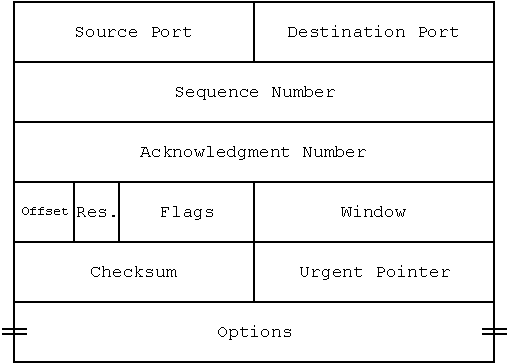
\includegraphics[page=1,scale=0.9]{TCPHeader.pdf}
\end{center}
\begin{itemize}
\item \texttt{Source Port}(16Bits): Identifica el puerto de origen del proceso de solicitud en el dispositivo emisor.
\item \texttt{Destination Port}(16Bits): Identifica el puerto de destino del proceso de solicitud en el dispositivo receptor.
\item \texttt{Sequence Number}(32Bits): número de secuencia de bytes de datos de un segmento en una sesión.
\item \texttt{Acknowledgement Number}(32Bits): cuando se activa el indicador \texttt{ACK} este numero contiene el siguiente numero de secuencia del byte de datos esperado y funciona como \texttt{ACK} de recibo de los datos recibidos anteriormente.
\item \texttt{Data Offset}(4Bits): este campo implica tanto el tamaño del encabezado TCP (palabra de 32 bits) como el desplazamiento de datos en el paquete actual en todo el segmento.
\item \texttt{Reserved}(3Bits): Reservado para uso futuro y todos están configurados en 0 de manera predeterminada.
\item \texttt{Flags}: indicadores de bits que indican como debe intepretar.
\begin{itemize}
\item \texttt{SYN}: Es usado durante el establecimiento de la conexión.
\item \texttt{FIN}: Es usado durante la liberación de la conexión.
\item \texttt{RST}: Se usa en caso de problemas o cuando un segmento invalido es recibido.
\item \texttt{ACK}: Cuando se lo establece, indica que el campo de reconocimiento contiene un número valido. De lo contrario, el receptor debe ignorar el contenido del campo de reconocimiento.
\item \texttt{URG}: Es usado junto con el Urgent Pointer.
\item \texttt{PSH}: Cuando se establece, es una solicitud a la estación receptora para empujar datos (tan pronto como llegue) a la aplicación receptora sin almacenarlo en el buffer.
\item \texttt{CWB}: Cuando un host recibe un paquete con el conjunto de bits \texttt{ECE}, establece la reducción de congestión de ventana, para confirmar recibe \texttt{ECE}.
\item \texttt{ECE}: Tiene dos significados:
\begin{itemize}
\item Si el bit \texttt{SYN} es 0, entonces \texttt{ECE} significa que el paquete IP tiene establecido su bit \texttt{CE} (Congestion).
\item  Si el bit \texttt{SYN} se establece en 1, \texttt{ECE} significa que el dispositivo es compatible.
\end{itemize}
\end{itemize}
\item \texttt{Window}: Este campo se usa para el control de flujo entre dos estaciones o indica la cantidad de buffer (bytes) que el receptor ha asignado para un segmento, es decir \textbf{cuantos datos espera el receptor.}
\item \texttt{Checksum}: La verificación.
\item \texttt{Urgent Pointer}: apunta al byte de datos urgentes si el indicador esta en 1.
\item \texttt{Options}: opciones adicionales que no están cubiertos por el encabezado regular.
\end{itemize}
\subsection*{Addressing}
La comunicación \texttt{TCP} entre dos hosts remotos se realiza mediante numeros de puerto, van desde 0 a 65535:
\begin{itemize}
\item System Ports(0-1023)
\item User Ports(1024-49151)
\item Private/Dynamic Ports (49152-65535)
\end{itemize}
\subsection*{Gestión de la Conexión}
Funciona en el modelo Servidor/Cliente. El cliente inicia la conexión y el servidor la acepta o la rechaza. El protocolo de enlace de 3 vías (3 Ways Handshake) se usa para la administración de la conexión.\\${ }$\\
\noindent
\begin{minipage}[t]{.5\textwidth}
\raggedright
\subsubsection*{Establecimiento}
El cliente inicia la conexión y envía el segmento con un número de secuencia. El servidor lo confirma con su propio número de secuencia y \texttt{ACK} del segmento del cliente que es uno mas que el numero de secuencia del cliente. El cliente después de recibir \texttt{ACK} de su segmento envía una señal de recibo de la respuesta del servidor.
\subsubsection*{Liberación}
Tanto el servidor como el cliente pueden enviar un segmento con el indicador \texttt{FIN} establecido en 1. Cuando el extremo receptor responde con \texttt{ACK FIN}, se cierra y libera.
\end{minipage}% <---------------- Note the use of "%"
\begin{minipage}[t]{.5\textwidth}
\noindent
\raggedleft
\begin{center}
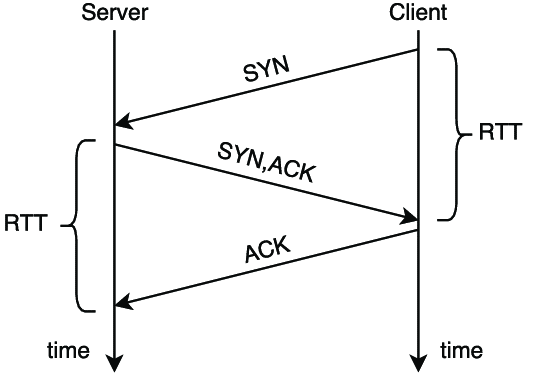
\includegraphics[scale=0.45]{3WAY.png}
\end{center}
\end{minipage}
\subsection*{Errores y Flujos}
Utiliza numeros de puerto para saber que proceso de aplicación necesita para transferir el segmento de datos. Junto con eso, utiliza un número de secuencia para sincronizar con el host remoto. Todos los segmentos de datos se envían y reciben con números de secuencia. El remitente sabe que ultimo segmento de datos recibió el receptor cuando recibe \texttt{ACK}. El receptor conoce el ultimo segmento enviado por el remitente al referirse al número de secuencia del recibido.
\subsection*{Control de Congestión}
Cuando llega una gran cantidad de datos al sistema que no es capaz de manejarlos se produce congestión. Controla esto por la ventana. Establece un tamaño de ventana que le dice al otro extremo cuantos segmentos de datos enviar, se usan tres algoritmos:
\begin{itemize}
\item Incremento Aditivo, Decremento Multiplicativo\
\item Slow Start
\item Timeout React
\end{itemize}